
In \fref{chap:intro} I have argued that the use of the MMSE in a filtering problem is an appropriate measure for the quality of a neural encoder in a dynamic setting. In 
this chapter I will consider a neural population as an encoder, seeking the tuning functions for that population that minimise the decoding error.
I will focus especially on the case of dense populations of Gauss-Poisson neurons. For these populations I will consider the class of
linear stochastic processes described in \fref{chap:filtering} and \fref{chap:mse} and investigate the dependence of the MMSE for those processes on the encoder's 
parameters. In the case of dense populations of Gauss-Poisson neurons I will argue that it makes the most sense to consider the width of the tuning functions as the central parameter 
of the encoder. I have found that for this type of population of neurons there is a finite optimal tuning width which minimises the
MMSE of the filtering problem.\par

Following the investigation, I also present an analysis of dense populations of Gauss-Poisson neurons coding for more complex stochastic processes, such as bistable
processes. In this setting, the filtering equations cease to be Gaussian, and one is forced to use approximate filtering to obtain estimates of the MMSE.
I have used both the ADF approach with a Gaussian density and a simple particle filter and show results for both cases, which also show that a finite tuning width minimises
the MMSE.\par

Finally, I will discuss some results comparing optimal population codes for filtering and control. In a set of examples, the
optimal encoders for an estimation and the associated control problem are different. This is the first result of this kind to the best of my knowledge.\par

There has been a lot of interest in the relation between the coding mechanisms in sensory systems and the statistics of the natural environment these systems operate in. A number of
studies have shown that one can obtain coding strategies similar to the ones employed by sensory systems as optimal codes for a natural ensemble of stimuli. For example, by
optimising linear filters for reconstruction of naturalistic visual stimuli under sparsity constraints, Olshausen and Field have obtained a set of filters which resemble the receptive
fields of V1 pyramidal neurons.\mycite{Olshausen1996,cadieu2008} Though the analysis presented here is somewhat simplistic, I believe it provides a solid foundation for similar studies
of reconstruction-based analysis of optimal codes. Similar approaches have been used in the literature, but there the focus was usually on static stimuli.\mycite{berens2012,Yaeli2010}
A notable exception is the work of \mycitep{Bobrowski2009}, where a formalism of full-spike train decoding was presented for finite-state dynamic systems. In a certain sense,
this work is an extension thereof to the case of continuous stimuli in continuous time. The present approach also makes the study of control problems a natural extension. The
issue of optimal coding for control problems has been widely overlooked, and this approach is novel to the best of my knowledge.\par

\section{Filtering through Point Processes and Optimal Codes}

Though I have introduced the general picture in \fref{chap:filtering}, I will shortly contextualise the framework again. I am interested in modelling a cortical area which is observing spike
trains from a population of upstream neurons $N^i(t)$, whose rates depend on a stochastic process $X(t)$ through tuning functions $\lambda^i(x)$. The objective is to estimate the 
state $X(t)$ from the observations
$\boldsymbol{N}(t) = \{N^i(t)\}$ as precisely as possible. Furthermore, I am interested in finding the set of tuning functions $\lambda^j(x)$ driving the observation processes that minimise 
the MMSE of the estimator $\hat{X}(\boldsymbol{N}_{0:t})$. I will denote the parameters of the encoder by $\varphi$.\footnote{In the case of a population of Gauss-Poisson neurons, 
the parameters are given by $\varphi = \{\{\theta_i\}, \covar, \phi\}$.} The optimal encoder is the encoder that minimises the MMSE, which is given by the set of parameters $\varphi^*$,
such that
\begin{align*}
\varphi^* =& \argmin_\varphi \boldsymbol{E}\left[\Tr\left[\left(X(t) - \hat{X}(\boldsymbol{N}_{0:t})\right)\left(X(t) - \hat{X}(\boldsymbol{N}_{0:t})\right)^\top \right]\middle| X, \boldsymbol{N},\varphi\right]\\
=& \argmin_\varphi \Tr\left[\epsilon(\varphi)\right].
\end{align*}
Note that differently from \fref{chap:mse} I am considering the trace of the MMSE matrix here. This is done to obtain a scalar measure of the quality of a
multidimensional estimation problem. The trace gives the sum of the eigenvalues of the MMSE matrix, providing a practical measure of how far from the true value
the estimator is on average. In the second line I have also dropped the time dependence as I will be mostly considering stationary results for the MMSE.
\par

\begin{figure*}
\label{fig:filtering_expl}
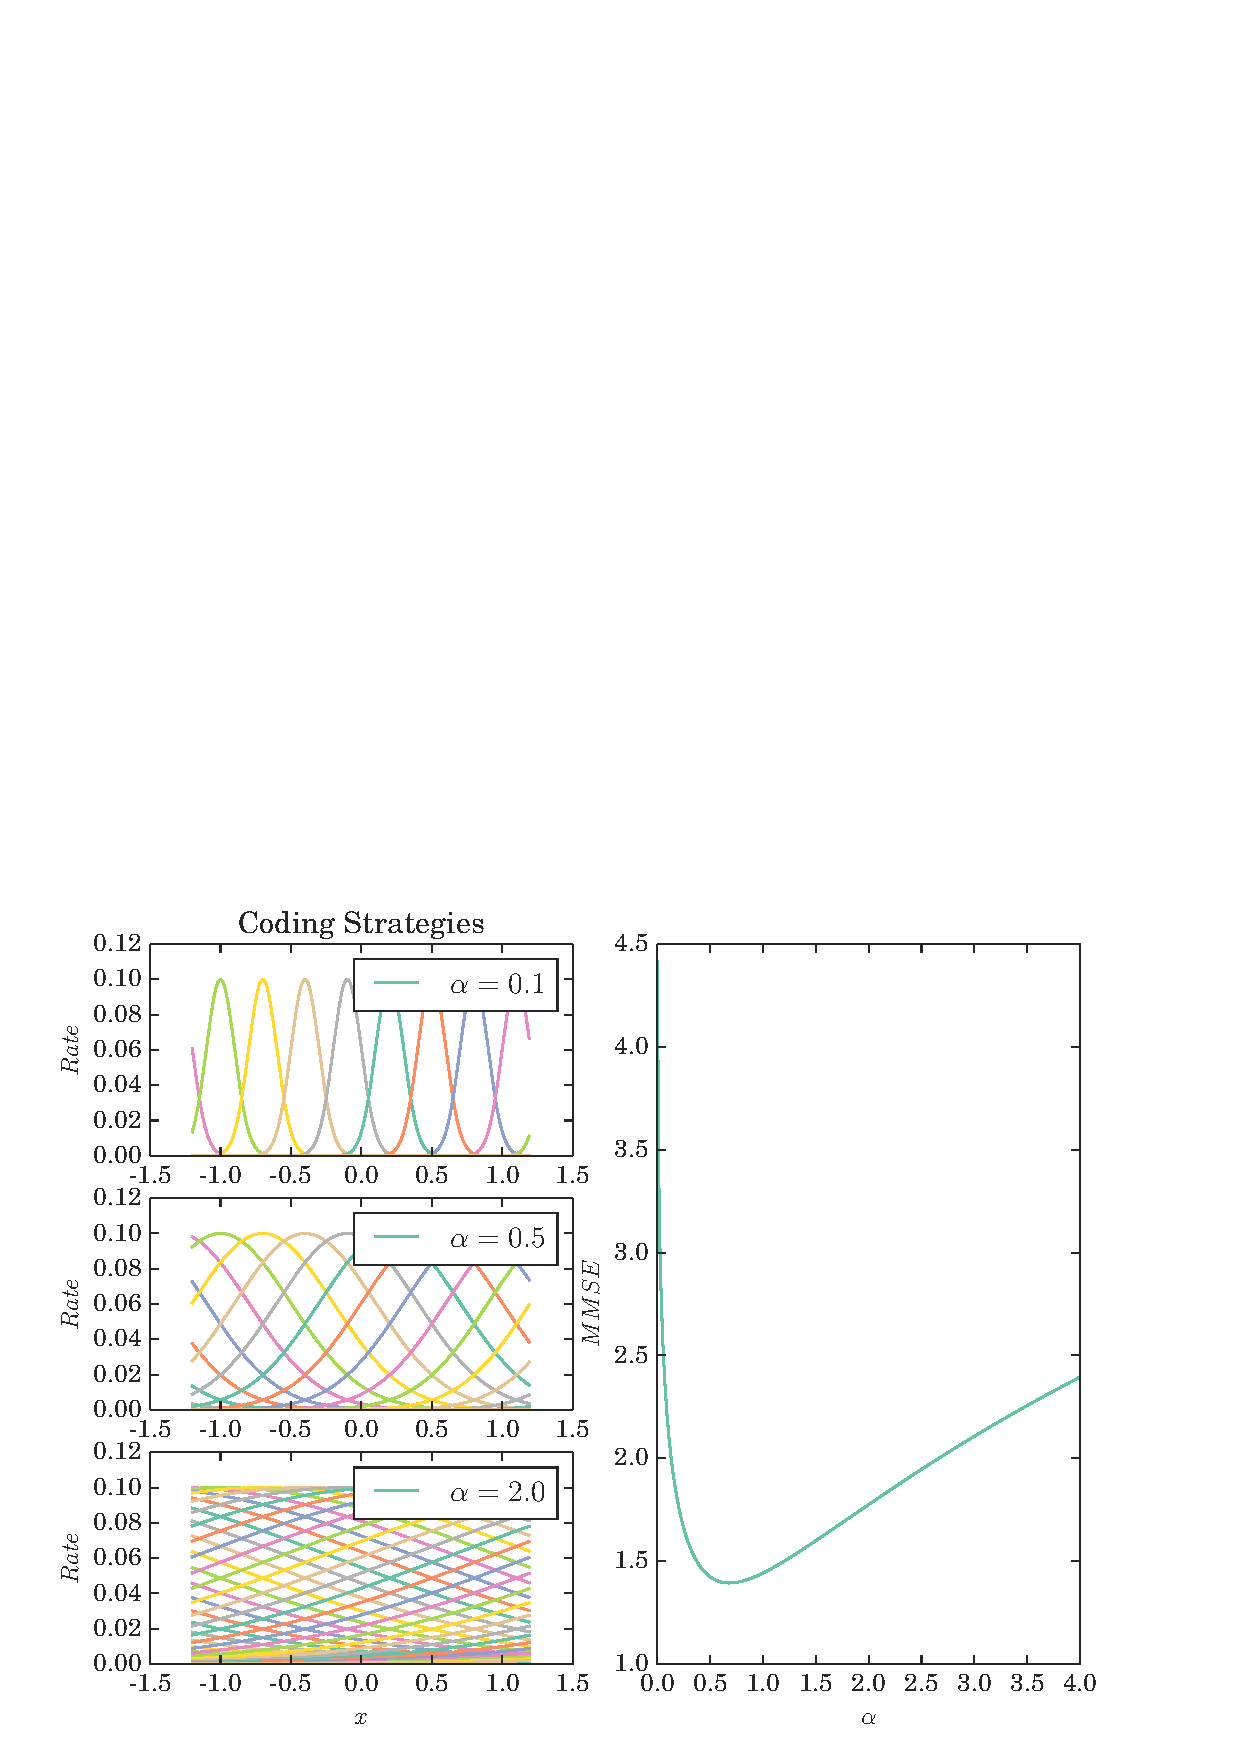
\includegraphics[width=\columnwidth]{figures/figure_5_1.pdf}
\caption[Optimal coding for filtering.]{Optimal coding for filtering Problems: The leftmost column shows the tuning curves of the neurons in the population. Meanwhile, the middle column
shows the general setup of the filtering scheme for each population for the same stochastic process. Note the different situations for narrow and broad tuning curves.
The rightmost plot shows the MMSE as a function of the tuning width $\alpha$.}
\end{figure*}

\subsection{Optimal Codes for Control}

In \fref{chap:control} I have introduced the formalism of stochastic optimal control and shown how to extend it to deal with point process observations. In a similar way
as one can define an optimal encoder for a filtering problem, one can define an optimal encoder for a control problem. Given a control problem with a cost function
\[
C(\boldsymbol{N}_{[0,T]},U_{[0,T]}) =\boldsymbol{E}\left[ \int_0^T c(X(t),U(\boldsymbol{N}_{[0,t]})) dt\mid \boldsymbol{N}\right],
\]
one can define the optimal encoder to be the one with parameters $\varphi^*$ given by
\[
\varphi^* = \argmin_\varphi C(\boldsymbol{N}_{[0,T]},U_{[0,T]};\varphi).
\]
This can lead to different results than the filtering framework as  I will show below.\mycite{Susemihl2014}\par

\subsection{Dense Gauss-Poisson Populations}

In this chapter I will mostly discuss results regarding dense populations of Gauss-Poisson neurons. So, unless otherwise noted, I am discussing a population of Poisson neurons
with tuning functions $\lambda^m(x)$ given by
\begin{equation}
\label{eq:tuning_function}
\lambda^m(x) = \phi \exp\left[-\frac{1}{2} (x-\theta_m)^\top \covar^\dagger (x-\theta_m)\right].
\end{equation}
When the stimulus is one-dimensional, I will denote the covariance of the tuning function by $\alpha$ instead of $\covar$.\par
The dense coding property holds if the overall firing rate of the population $\hat{\lambda} = \sum_i \lambda^i(x)$ is independent of the stimulus $x$. I will refer to a population
of Poisson neurons with Gauss tuning functions such that the dense coding property holds as a dense population of Gauss-Poisson neurons.


\section{Filtering Linear Stochastic Processes through dense Gauss-Poisson Spike Trains}

Consider a linear stochastic process of the type
\[
dX(t) = AX(t) + H^{1/2} dW(t).
\]
Though this may seem as a somewhat restrictive choice, a number of processes can be cast into this format. The simple Ornstein-Uhlenbeck process, which I considered in
previous chapters is one example, but generalisations to higher dimensions are relatively simple and include, for example, the stochastic damped oscillator. The matrices
\[
A= \left(\begin{array}{cc} 0 & 1\\ -\omega^2&-2 \gamma\end{array}\right), \textrm{ and }H= \left(\begin{array}{cc} 0 & 0\\ 0& \eta \end{array}\right),
\]
will lead to a stochastic process with a periodic component, more precisely the stochastic damped oscillator given by the system of SDE's
\[
\dot{X}(t) = V(t), \quad dV(t) = -2 \gamma V(t)dt -\omega^2 X(t) dt + \eta dW(t). 
\]
I have here written a pre factor of $2$ to the damping coefficient, so that the choice $\gamma = \omega$ leads to the critically damped stochastic oscillator.
This is an example of embedding a non-Markov one-dimensional process in a higher-dimensional space to recover the Markov property, as described in \fref{sec:stochastic_proc}.
In \fref{fig:stoch_example} a few examples of linear stochastic systems are shown, with a couple of 
random samples of each per plot. Although the focus here is on stationary stochastic processes,
this is by no means a necessity for the analysis at hand. Even for non-stationary processes such as the Wiener process,\marginnote{The Wiener process $W(t)$, for example, has
a covariance that increases linearly with time.} the posterior density can be stationary, allowing us to evaluate the stationary MMSE.\par

\begin{figure}
\label{fig:stoch_example}
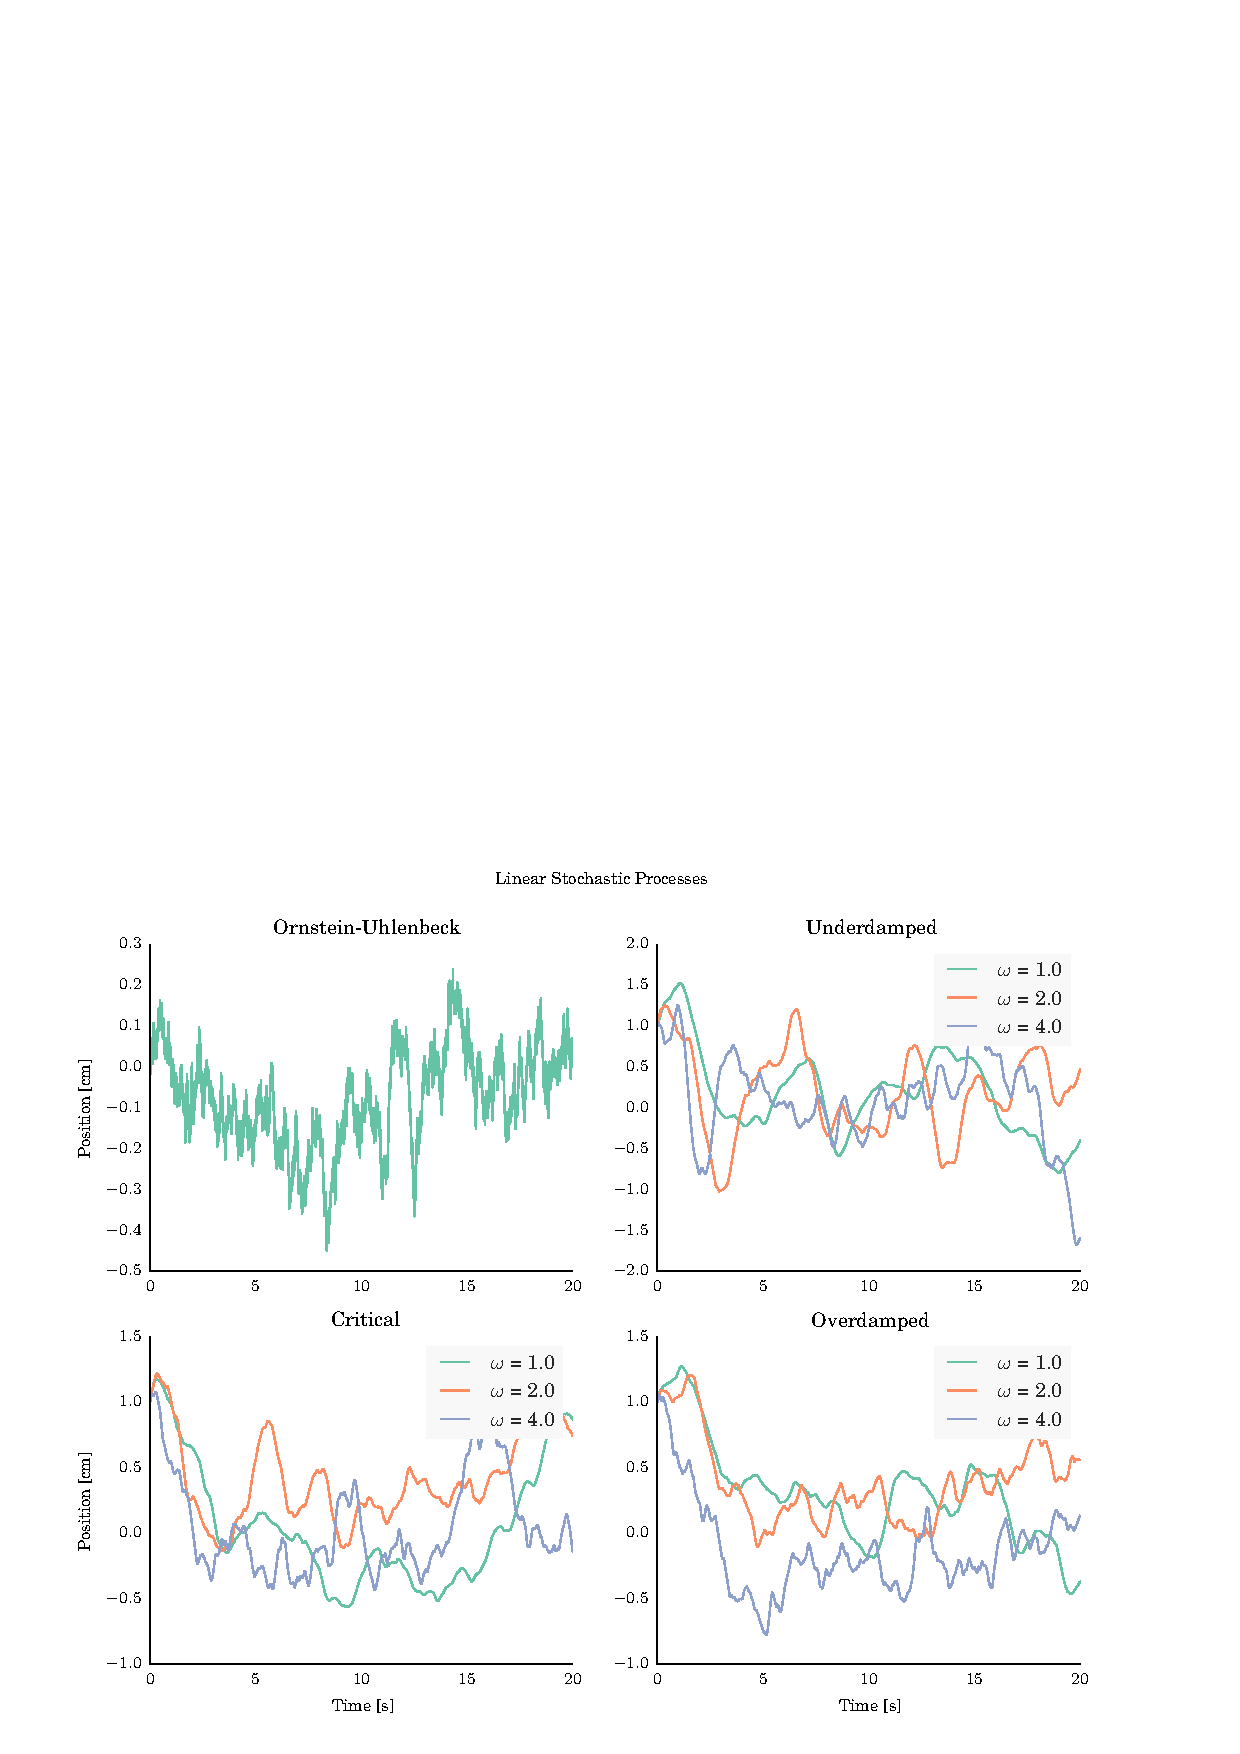
\includegraphics[width=\columnwidth]{figures/figure_5_2.pdf}
\caption[Samples of linear stochastic processes.]{Linear stochastic processes: From the top left, we have the one-dimensional Ornstein-Uhlenbeck process, an underdamped stochastic oscillator,
a critically damped stochastic oscillator (bottom left), and an over damped stochastic oscillator.}
\end{figure}


The MMSE $\epsilon(t)$ can be obtained from the formalism derived in \fref{chap:mse}. Throughout this section I will use both the numerical solution of the
evolution equations for $\epsilon(t)$ as well as the mean-field approximation to it.\par

Let me start with the simplest stationary stochastic process, the Ornstein-Uhlenbeck process
given by
\[
dX(t) = -\gamma X(t) dt + \eta^{1/2} dW(t),
\]
where the exact evolution of the MMSE is given by
\[
\frac{d\epsilon(t)}{dt} = -2\gamma \epsilon(t) + \eta -\hat{\lambda} \boldsymbol{E}\left[\frac{s^2}{\alpha^2+s}\right].
\]
I will not consider the temporal evolution of the MMSE, instead
I will focus on the stationary value of the MMSE, and therefore on the long-term performance of the encoder in the filtering problem, rather than focusing
on the transient, short-time behaviour. I am mostly interested in the dependence of the optimal encoder in the statistical structure of the stimulus, i.e. the correlation
timescales and the noise levels. In a natural environment, these changes should be generally slower than the adaptation processes of the sensory apparatus. This is my main
motivation to focus on the stationary regime.\par
In \fref{fig:mmse_ou} the equilibrium MMSE of a dense Gauss-Poisson population of neurons encoding
an OU process is shown. The dependence on both the maximal firing rate $\phi$ and the tuning width $\alpha$ is shown.

\begin{figure*}
\label{fig:mmse_ou}
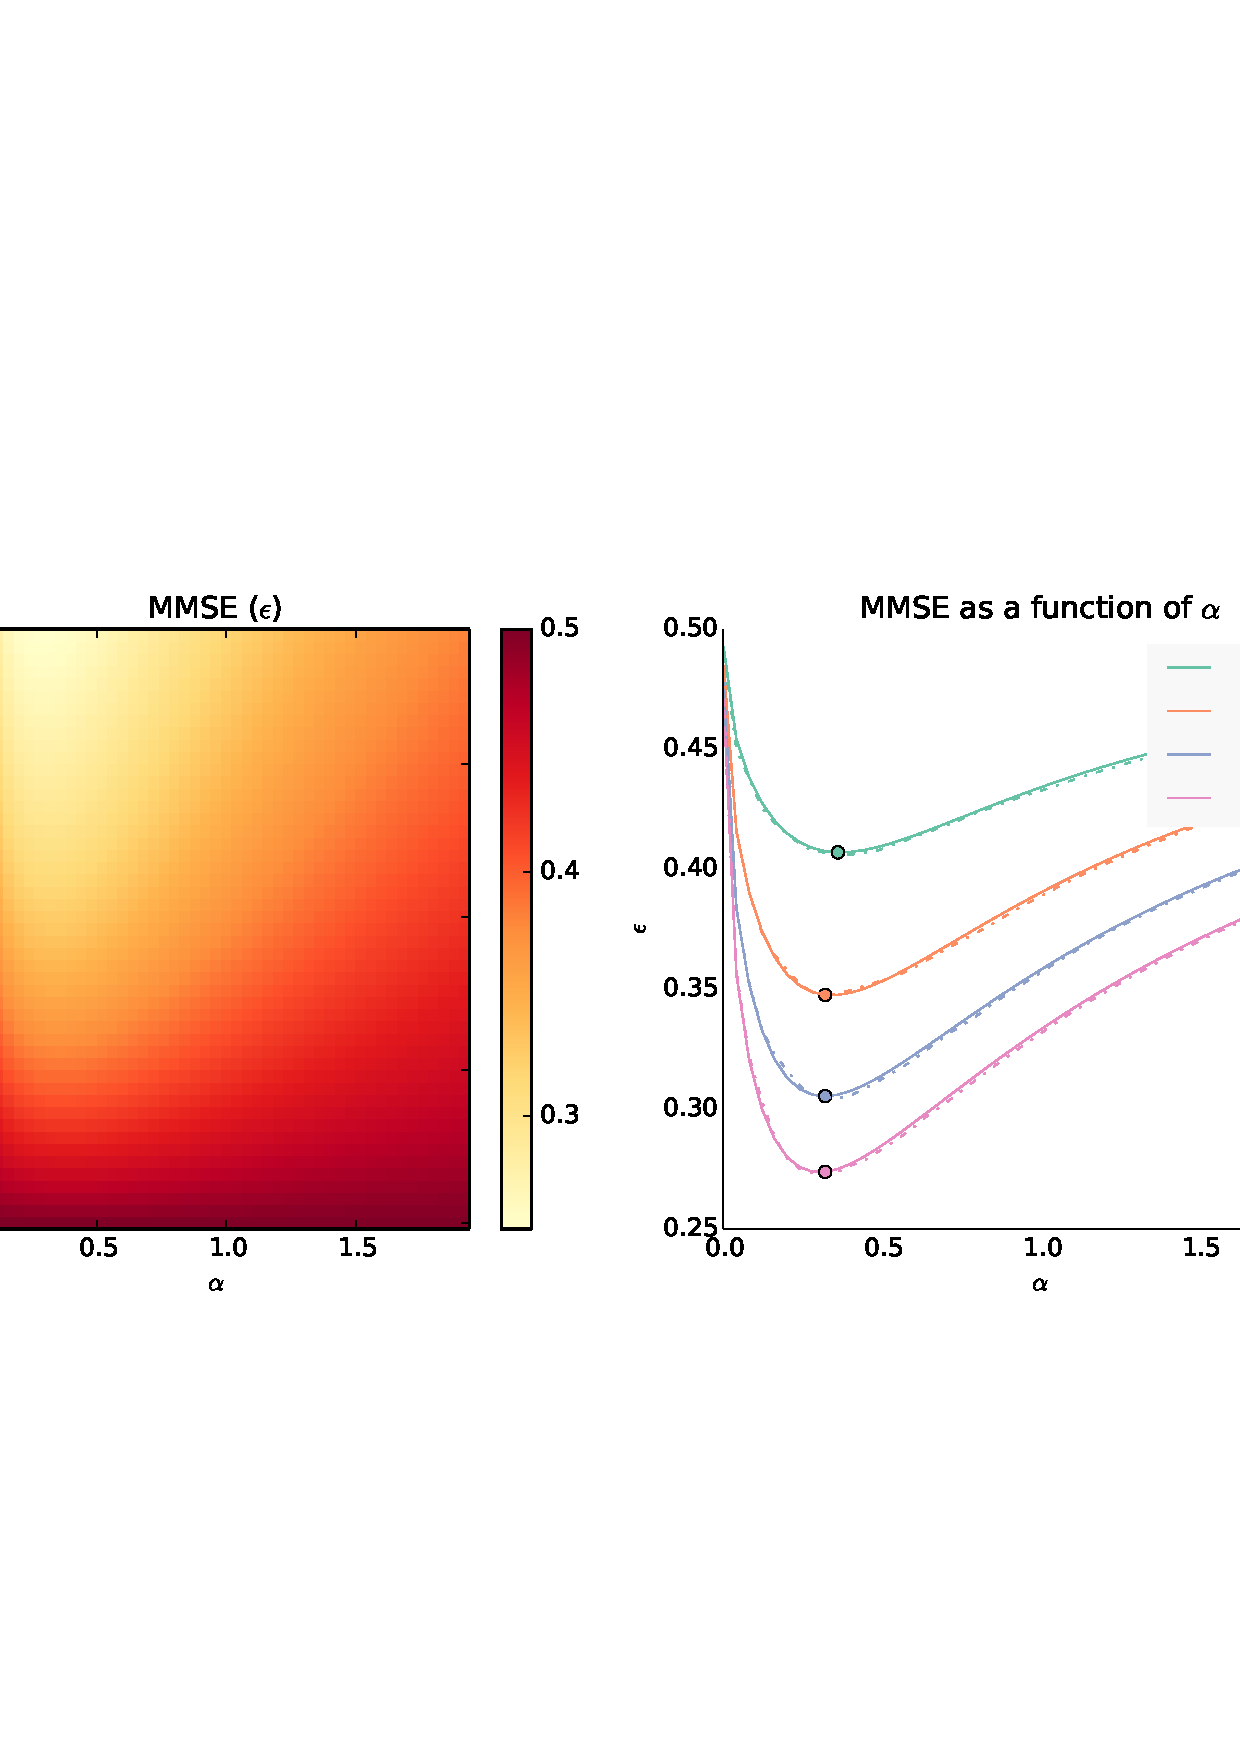
\includegraphics[width=\columnwidth]{figures/figure_5_3.pdf}
\caption[Optimal encoding for the OU process.]{Comparing Encoders for Filtering: The left hand panel shows a heat map of the MMSE as a function of the maximal firing rate $\phi$ and the tuning
width $\alpha$. There is a trade-off between the number of spikes and the precision of the spikes, manifesting itself in a finite tuning width that minimises the
the MMSE. For any $\alpha$ increasing the firing rate $\phi$ simply decreases the MMSE. The right panel shows the dependence in $\alpha$ for a few values
of $\phi$.}
\end{figure*}

More interestingly, one can now ask how the optimal encoder depends on any of the parameters of the problem, such as the parameter $\gamma$, for example,
which defines the time-scale of correlations in the OU process.\footnotemark
In \fref{fig:ecological_ou} I have plotted the optimal encoding width $\alpha^*$ as a function of $\gamma$, $\eta$ and
$\phi$. It is interesting to be able to provide an accurate account of the dependence of the optimal 
encoder on the statistical structure of the environment. The leftmost panel shows the dependence of the optimal tuning width in $\gamma$. Shorter time-scales (larger values of $\gamma$) require a higher frequency of spikes, as the information conveyed by those spikes becomes irrelevant
more quickly.\footnotetext{Remember that the prior kernel of the OU process is given by $k(s,t) = \frac{\eta}{2\gamma} \exp(-\frac{|s-t|}{2\gamma})$.} Thus, holding the maximal firing rate $\phi$ fixed, the only way to increase the frequency of spikes is to have broader tuning functions. Therefore, as $\gamma$
increases, so does $\alpha^*$. Likewise, a higher noise rate $\eta$ leads to the need for more spikes to characterise the system's state, leading to higher values
of $\alpha^*$. Increasing the maximal firing rate $\phi$ of the neurons, on the other hand, leads to smaller optimal tuning widths $\alpha^*$.


\begin{figure}
\label{fig:ecological_ou}
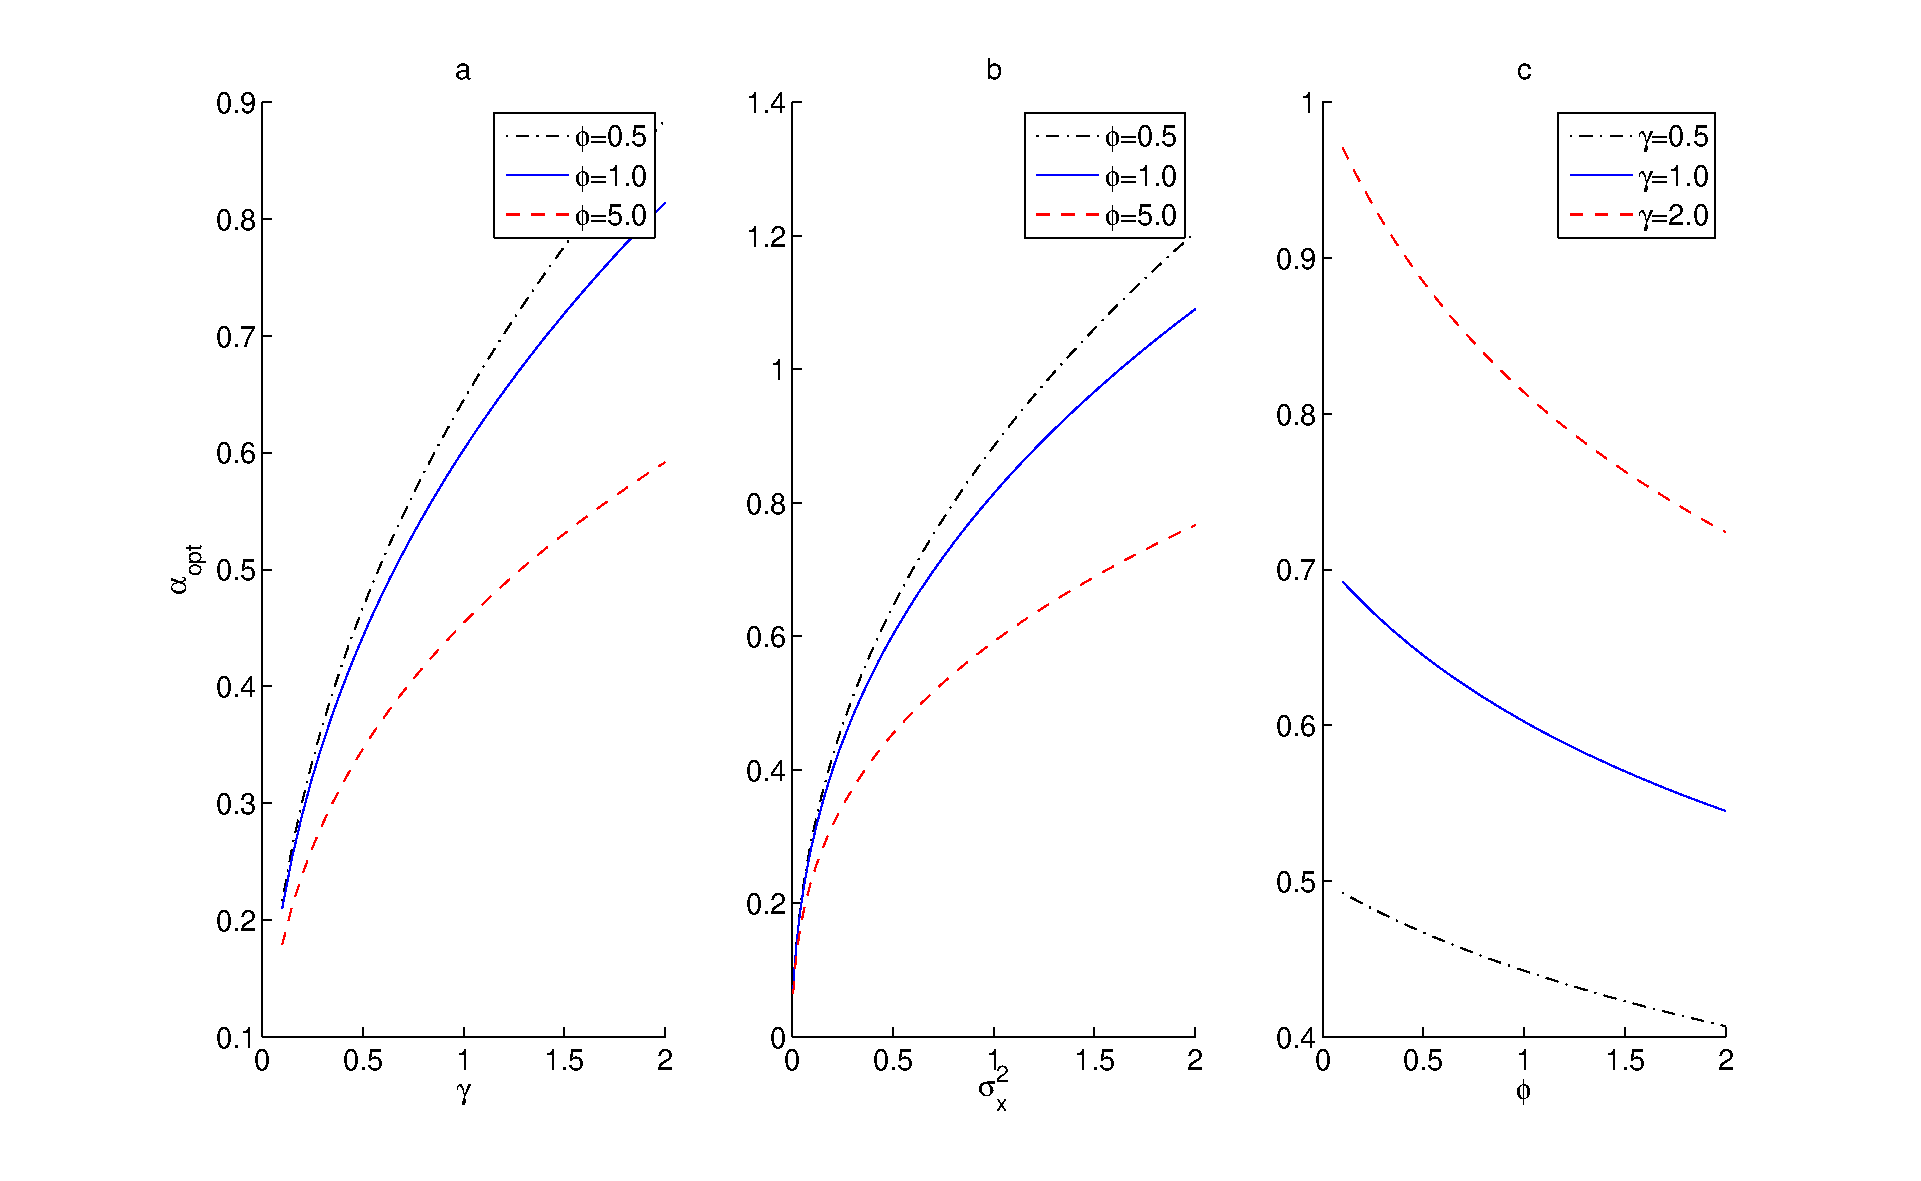
\includegraphics[width=\columnwidth]{figures/figure_5_4.eps}
\caption[Ecological dependence of the optimal encoder.][50pt]{Ecological Dependence of the Optimal tuning width for a dense population of Gauss-Poisson neurons encoding the state of an OU process. Increasing the timescale of the correlations $1/2\gamma$ leads to smaller optimal tuning widths, this can be seen in (a). (b) An increase in the noise rate of the process leads to larger optimal
tuning widths, as an increase in the variance of the process requires more observations to characterise it. (c) The maximal firing rate of each neurons $\phi$ sets the tradeoff
between frequency and precision of the observations. A higher firing rate, tilts the tradeoff towards more precise observations, leading to smaller optimal tuning widths. }
\end{figure}

\subsection{Stochastic Harmonic Oscillator}
A natural extension to consider is the same setup but with the stimulus given by the stochastic harmonic oscillator presented above. Here I will consider a population of neurons whose
firing rate depends only on the position of the oscillator, not on the velocity. This would be equivalent to taking the tuning matrix
\[
\covar = \left(\begin{array}{cc} \alpha^2 & 0\\0&0\end{array}\right),
\]
leading to the same form of the tuning functions as before.
The results are very similar to the OU case, 
regardless of the smoother nature of the process considered. In \fref{fig:mmse_osc} the MMSE for a dense Gauss-Poisson population coding for
a stochastic oscillator is shown. Likewise, \fref{fig:ecological_osc} presents the dependence of the optimal tuning width on the parameters of the encoder and the environment.
There are three parameters determining the dynamics of the environment, the frequency $\omega$, the damping $\gamma$ and the noise rate
$\eta$, and I have presented the dependence of the optimal tuning width on all three. Interestingly, in \fref{fig:ecological_osc} (c), one can note a quite different behaviour for the
stochastic oscillator. The case $\gamma=0.5$ represents an underdamped oscillator, $\gamma=1$ is the critically damped oscillator and $\gamma=5.0$ an over damped oscillator.
First one can note that the dependence of the optimal tuning width on the firing rate $\phi$ is much less pronounced than in the OU process. This is to be expected, as the stochastic
oscillator has a smoother structure, and allows one to predict it from past observations more reliably. It can also be noted that the effect of increasing the firing rate on the optimal
tuning width is strongest in the underdamped regime, which can also be understood by looking at \fref{fig:stoch_example}. When increasing the damping coefficient $\gamma$, the
stochastic variations in the velocity become smaller, and the system's state $X(t)$ has smaller, shorter time-scale variations around $X(t)=0$, while the overall variance of the process
also becomes smaller.

\begin{figure*}
\label{fig:mmse_osc}
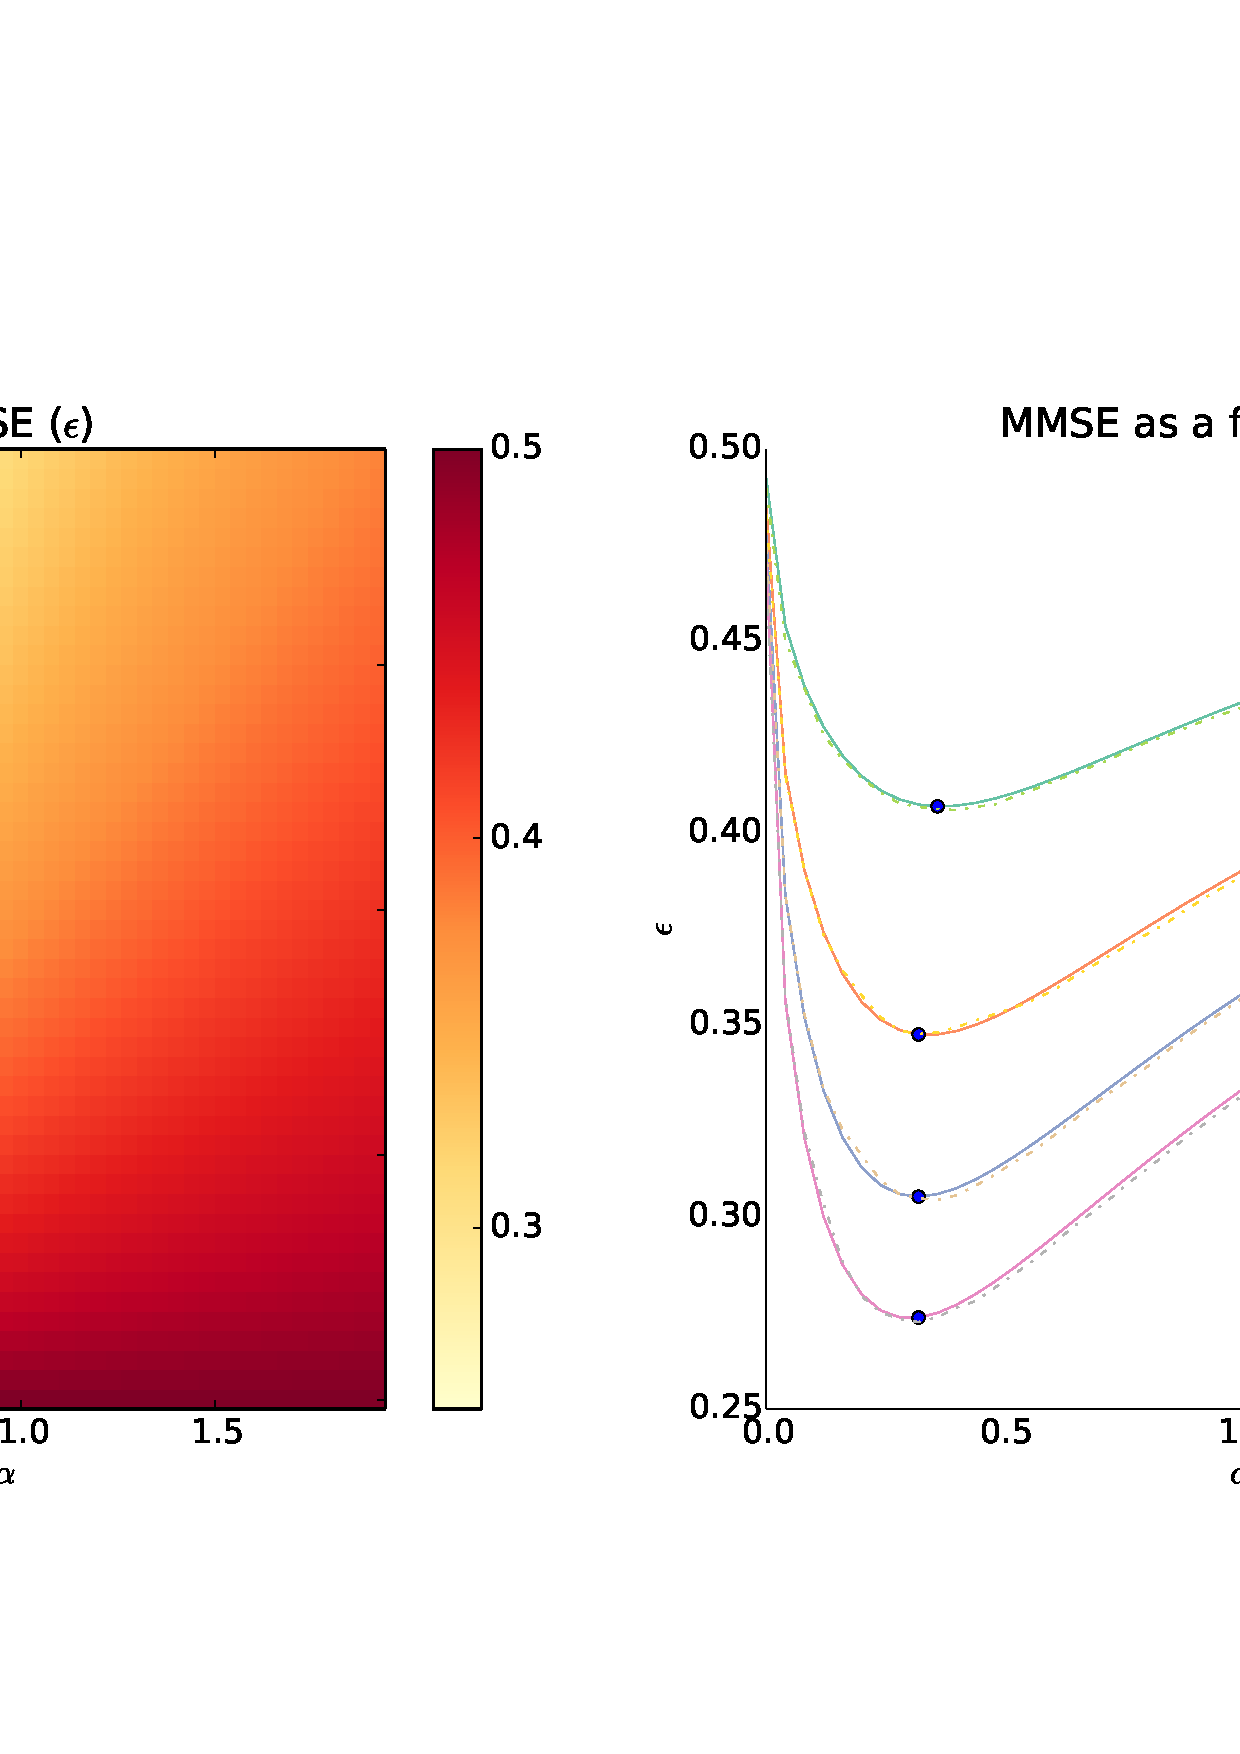
\includegraphics[width=\columnwidth]{figures/figure_5_5.pdf}
\caption[Optimal encoders for the stochastic harmonic oscillator.]{Comparing Encoders for Filtering: The left hand panel shows a heat map of the MMSE as a function of the maximal firing rate $\phi$ and the tuning
width $\alpha$. There is a trade-off between the number of spikes and the precision of the spikes, manifesting itself in a finite tuning width that minimises the
the MMSE. For any $\alpha$ increasing the firing rate $\phi$ simply decreases the MMSE. The right panel shows the dependence in $\alpha$ for a few values
of $\phi$.}
\end{figure*}

\begin{figure}
\label{fig:ecological_osc}
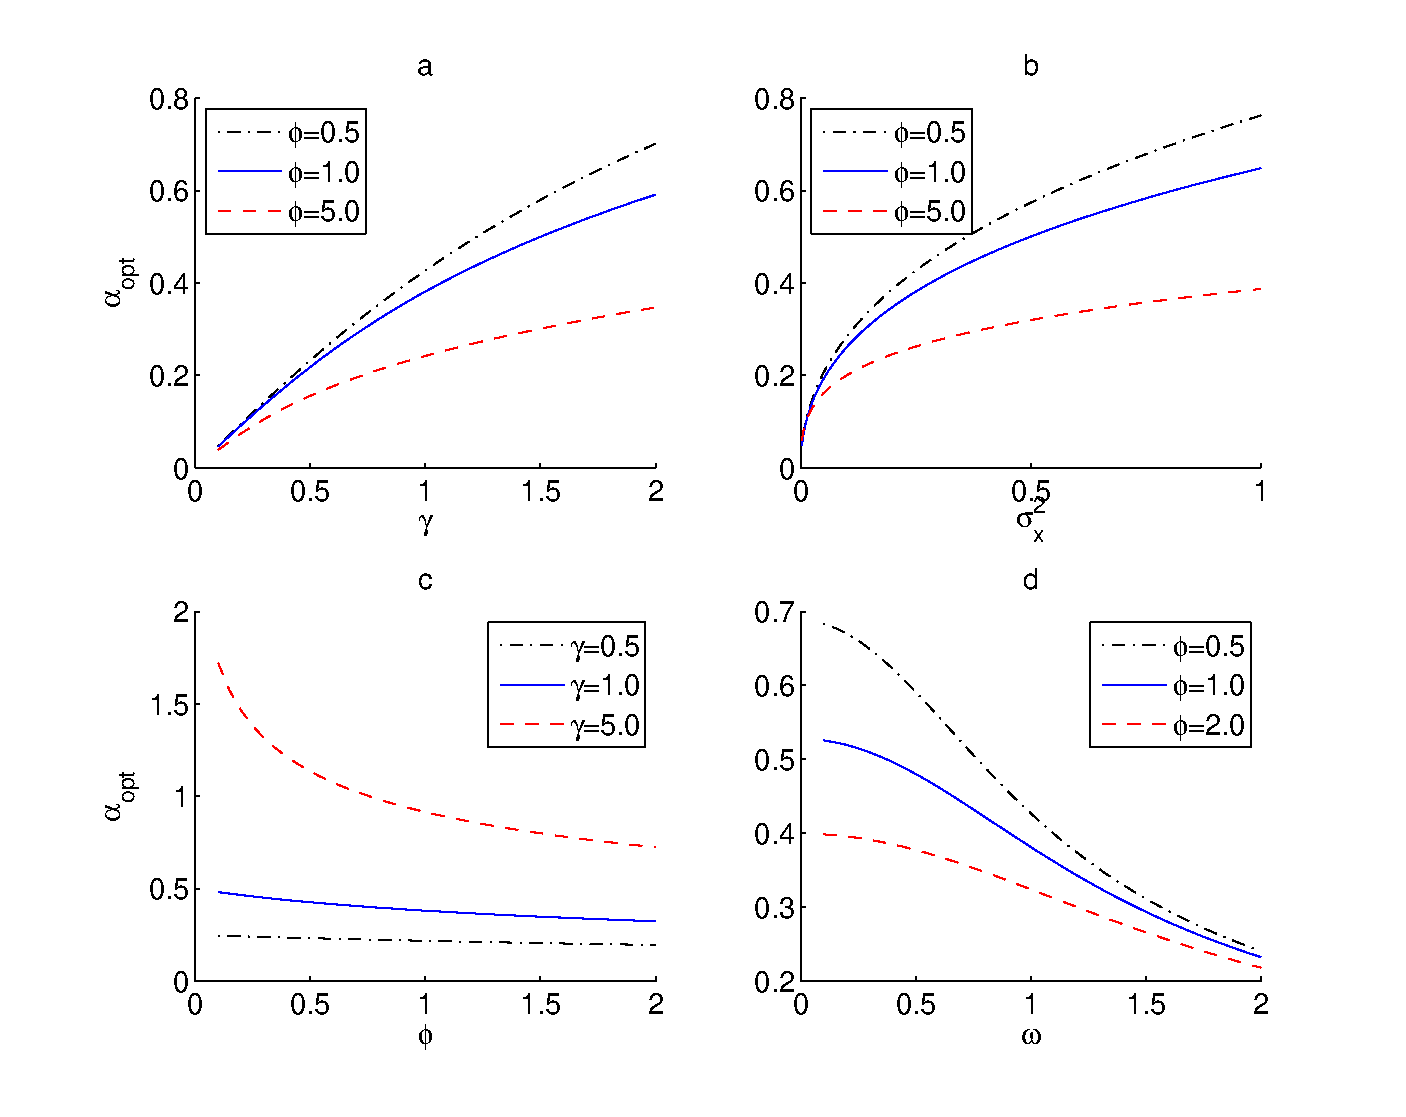
\includegraphics[width=\columnwidth]{figures/figure_5_6.eps}
\caption[Ecological dependence of the optimal encoder for the stochastic oscillator.][50pt]{Ecological Dependence of the Optimal tuning width for a dense population of Gauss-Poisson neurons encoding the position of a stochastic oscillator. The effect of the damping is similar to the effect of the
parameter $\gamma$ in the OU case, as it sets the time-scale of fluctuations in the velocity, which in turn drives the position being estimated. Lower $\gamma$ lead to longer time correlations in the velocity and also in the position, leading to easier reconstruction and a narrower optimal tuning width. The noise intensity $\eta$ also has the same effect as in
the OU process, as a stronger noise leads to wider optimal tuning widths. The maximal firing rate of each neuron $\phi$ has a much less pronounced effect on the optimal tuning width
than in the OU case, specially for the critical and overdamped regime. This is due to the smoother nature of these processes. The  frequency of the process, surprisingly, has the 
inverse effect as the damping, with higher frequencies leading to lower optimal tuning widths. This is due to the damping effect it has on the velocity, leading to a shorter integration
time for the noise in the velocity.}
\end{figure}

\subsection{Smooth Processes}

Through the kernel process formulation developed in \fref{sec:kernels} one can also treat general Gaussian processes, even non-Markov ones such as the RBF process.
By non-Markov processes, I mean processes which can not be rendered Markovian by the inclusion of its derivatives in a higher-dimensional embedding.
The MMSE is given by the average posterior variance of the Gaussian process regression, $\boldsymbol{E}_{\{t_i\}}\left[\Xi(t,t;\{t_i\})\right]$, which can be approximated by the 
mean-field posterior kernel $g(0)$.\footnote{See \fref{sec:kernels} and \fref{app:kernel_integral}.}
In \fref{fig:mmse_rbf} I have evaluated the kernel mean-field approximation for the RBF kernel $k(s,t) = \exp\left(-(s-t)^2/L\right)$, with $L= 0.5$. Note that the general
conclusions drawn in the two previous cases hold here as well, regardless of the more complex temporal structure of the process.\par

In the case of linear stochastic processes, I had found that the temporal mean-field approximation of \fref{eq:eps_mf} was surprisingly good at describing the average
behaviour of the posterior variance. Therefore it is interesting to study how the mean-field approach performs in the RBF case, where the filtering error is derived from
an approximation to the posterior kernel. To that intent, I can evaluate the average posterior variance from \fref{sec:kernels} numerically.
This can be done by generating a large number of Poisson spike trains and evaluating the posterior covariance $\Xi(t;\{t_i\})$ for each and taking an average.
This is also shown in \fref{fig:mmse_rbf} as the dotted lines.
The averaging in this case is much more costly, as for every set of $M$ spike times, one needs to invert an $M\times M$ matrix, which takes of the order of $M^3$ operations.
As can be seen from the figure, the mean-field approximation still agrees very well with the numerical average, leading to undistinguishable optimal tuning widths.

\begin{figure*}
\label{fig:mmse_rbf}
\includegraphics[width=\columnwidth]{figures/figure_5_7.pdf}
\caption[Optimal encoders for the RBF process.]{MMSE for a dense population of Gauss-Poisson neurons encoding a RBF process. The MMSE follows the same trends as for the OU process and the stochastic
harmonic oscillator. The dotted lines show the numerically averaged MMSE, obtained directly from the Gaussian process regression.}
\end{figure*}

\section{Moving Away From Gaussian Distributions}

In \fref{chap:filtering} I have presented filtering tools for general stochastic processes and observation processes, namely the ADF and particle filter techniques.
So far, in the analysis of optimal codes I have restricted myself to the dense coding limit, which significantly simplifies the analysis, rendering the Gaussian ADF approach
exact. What happens when the posterior is not Gaussian, though? I will consider a couple of interesting cases shortly. There are two ways one can leave the dense
coding limit. The first one is to have a population which does not densely cover the stimulus space. The simplest case would be a single neuron with a Gaussian tuning function,\footnotemark for example,
which could clearly not cover the stimulus space. The second possibility refers to the nature of the neurons. If their spiking is time-dependent or adaptive,\footnotetext{See \fref{fig:neuron_example}.} the homogeneity of the firing
rate will break and we will have a stimulus-dependent population firing rate as well. Of course the posterior can also be non-Gaussian due to the prior. That would mean the
process being observed is non-Gaussian. I will consider the simple case of a stochastic process in a double-well potential, as an example of non-Gaussian processes.
\par

Once again my main interest is in the optimality of said codes. It is straightforward to estimate the MMSE of the mentioned cases from simulations directly. 
Though much less practical than the dense coding case, where one could refrain from simulating the stimulus trajectories and spike trains, the principles remain the
same. It is not true, however, that the average posterior covariance gives the MSE of the estimator in this case. Remember that I have used that the estimator is the
posterior average to show that, and this does not hold generally for either the ADF or the particle filter estimator. For the particle filter, it can be shown that
in the limit of many particles the empirical distribution converges to the posterior distribution, yielding the posterior mean estimator in the limit of infinite particles.\mycite{crisan2002} 
The ADF estimator, however, has no simple relation to the posterior mean estimator, and further has no guarantee of converging to the true posterior. So in both cases we are forced 
to work directly with the average estimation error to obtain a measure of the MSE.\par

This section is meant to illustrate the application of the framework of MSE-optimal codes outside of the assumptions made in the previous section. Though optimising a code for
the MSE is not as straightforward for more complex, higher-dimensional problems, this shows that it is in principle possible, and the hurdles are mostly of implementation, rather
than conceptual.


\subsection{Sparse Populations}

The simplest form of breaking the dense coding assumption is, well, not having dense populations. The most extreme case would be if there were only one or
a few neurons coding for the stimulus. In that case, the population firing rate could be very strongly dependent on the state of the system. I will consider a simple
case here to illustrate the applicability of the MSE method. I will consider the case of a population of two neurons, equidistant from the mode of the stimulus distribution,
and investigate the dependence of the MSE on the separation between the two and the width of the tuning functions.\par

I will use three filtering schemes for this problem and compare them. First, I consider
the filtering equations given by \fref{eq:filtering_sdes}. In the dense coding case, these equations are exact, but one can use them as an approximate filtering method
regardless of the population being dense. This amounts to ignoring the probability of a spike not being fired, and looking only at the probability of a spike being fired when a spike is
actually observed. I will refer to this filtering scheme as the Dense ADF approach. A second possibility is to apply the ADF approach with a Gaussian distribution, now taking the rate 
terms in \fref{eq:adf_gauss_filter} into account and updating the mean and covariance through \fref{eq:gaussian_updates} upon the observation of a spike. I will refer to this option as 
the Full ADF approach. A third possibility is to use a particle filter with a large number of particle (I have taken $M=1000$ here) to estimate the posterior probability given the spikes.
This again, takes into  account the probability of a spike not having been fired in every time instant by every neuron.\par

%These approaches are compared in \fref{fig:dense_to_sparse} for a population of neurons separated by $\Delta\theta$ responding to a stimulus given by an OU process.
%As expected, when $\Delta\theta$ is very near zero, the schemes are virtually indistinguishable, however, as $\Delta\theta$ grows, the dense ADF approach gives a substantially
%larger MSE than the two other approaches, showing that this approach is only appropriate for small values of $\Delta\theta/\alpha$. Note that the MSE grows for all three approaches,
%since increasing $\Delta\theta$ lowers the overall firing rate, leading to fewer spikes, and therefore poorer MSE performance. The lowest MSE (therefore the one nearest the MMSE)
%is given by the particle filter, therefore I will choose to use the particle filter when no exact solution is obtainable. The Full ADF approach does not fare much worse, though, and it
%is still an interesting filtering method in practical applications as it does not require the simulation of multiple particles.\par
%
%\begin{figure}
%\includegraphics[width=\columnwidth]{figures/figure_5_15.pdf}
%\caption[Violating the dense coding assumption]{The violation of the dense coding assumption. As $\Delta\theta$ increases, the dense ADF approach performs poorly in comparison to the other two, showing the violation
%of the dense coding assumption. Of all three methods, the Particle filter shows the lowest MSE, therefore lending itself to an estimation of the MMSE.}
%\label{fig:two_neurons}
%\end{figure}
%

Assuming both neurons have Gaussian tuning functions with the same tuning width, one could ask
what is the best tuning width and spacing between the two neurons to optimise the MSE. In \fref{fig:two_neurons} I have plotted the MSE as a function of $\Delta\theta$ and
$\alpha$, showing a clear optimum. There are some artefacts due to the interplay of $\alpha$ and $\Delta\theta$, but all three approaches show a clear minimum. Surprisingly, even
in this case, the dense ADF approach yields nearly the same MSE as the particle filter or the full ADF approach, showing a relative absolute deviation from the full ADF approach of
less than 1\% and of approximately 1.5\% from the particle filter approach. This might be due to the Gaussian nature of the stimulus, but
it is an interesting point for further investigation.\par

\begin{figure}
\includegraphics[width=\columnwidth]{figures/figure_5_14.pdf}
\caption[Optimal coding with two Gaussian neurons.]{Two neurons with Gaussian tuning functions coding for a simple OU process. The left panel shows two sample tuning functions, explaining the parameters $\Delta\theta$ and
$\alpha$. The left panel shows the MSE according to the different approaches. The top shows the ADF approach assuming a dense population (i.e. ignoring the firing rates in the 
absence of spikes). The middle plot shows the MSE obtained with a full Gaussian ADF approach. The bottom plot shows the MSE of a particle filter. Though the three approaches
give different results, the general dependence of the encoder on the parameters is clear for all three approaches. There is an optimal value of $\Delta\theta$ and $\alpha$
which minimises the MSE in all three approaches}
\label{fig:two_neurons}

\end{figure}

\subsection{Adaptive Neurons}

A different situation which could lead to non-uniform firing rates is adaptation in the firing rate of the neurons, even in a dense population of neurons. The spike-frequency adaptation
process described in \fref{sec:ADF} is a simple model where the essence of neural adaptation is already present. I will consider the impact of adaptation
on the MMSE of a simple linear stochastic process as we have considered above.\par

\begin{figure}
\label{fig:adaptive_mse}
\includegraphics[width=\columnwidth]{figures/figure_5_8.pdf}
\caption[MSE of a population of adaptive neurons.]{The MSE of a reconstruction task from the observation of adaptive spike trains. The product $\tau\delta$ quantifies the intensity of the adaptation. As in the previous cases,
one can note the existence of a finite optimal tuning width.}
\end{figure}

A number of interesting questions arise with respect to adaptation in neurons. The adaptation implemented by the spike rate modulation $\kappa(t)$ is similar to the
spike-frequency adaptation often described in neuroscience.\mycite{benda2003} As can be seen in \fref{fig:adaptive_mse}, at first glance it
would seem that adaptation does not help the population code. This is somewhat misleading, though, as the stronger the adaptation time-scale $\tau$, the lower
the firing rate of the population. It would make sense, then to compare adaptive and non-adaptive populations with the same firing rate, to account for the effect of the
adaptation. This is shown in \fref{fig:adaptive_rate_distortion}. Here the mean-squared error of the filter is plotted as a function of the firing rate of the population, and it
is immediately obvious that the adaptive populations achieve a better performance with a much lower firing rate.\par

\begin{figure}
\label{fig:adaptive_rate_distortion}
\includegraphics[width=\columnwidth]{figures/figure_5_9.eps}
\caption[MSE for adaptive neurons as a function of population firing rate.]{MMSE of adaptive population as a function of the population firing rate. Though the adaptation leads to a worse reconstruction error when keeping all other parameters fixed,
here one can see that it allows for a more precise reconstruction with the same amount of spikes. There is a saturation in the improvement however, as the adaptation puts a limit
on the number of spikes the population can fire.}
\end{figure}

\subsection{Nonlinear Stochastic Processes}

A different source of non-Gaussian distributions can be found directly in the stochastic process one is modelling as stimuli. A simple model that leads to non-Gaussian
distribution is a stochastic process in a double well potentialo, given by $V(x) = \nu(x+x_0)^2(x-x_0)^2$. This potential will have two
stable points at $x=\pm x_0$. One can then define a stochastic 
system moving in this potential as
\[
dX(t)  = -\frac{dV}{dx}dt + \eta^{1/2} dW(t).
\]
This leads to
\[
dX(t) = 4\nu X(t)\left(x_0 - X(t)^2\right) dt + \eta^{1/2} dW(t).
\]
\Fref{fig:bistable_samples} shows some sample paths from this process.

\begin{marginfigure}
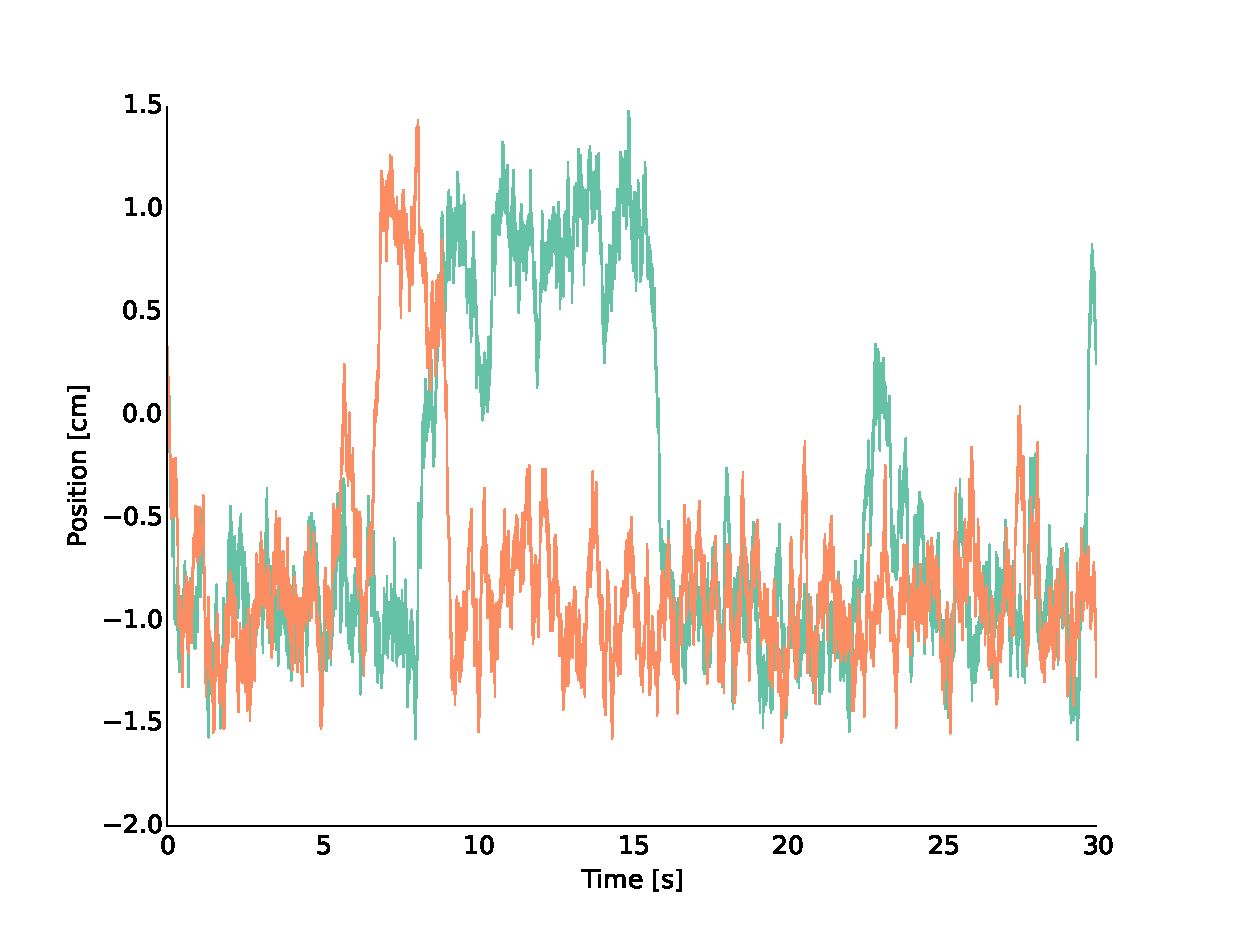
\includegraphics[width=\columnwidth]{figures/figure_5_10.eps}
\caption[Bistable Processes.]{Samples of the Bistable process mentioned in the text.}
\label{fig:bistable_samples}
\end{marginfigure}

Following the framework of \fref{chap:filtering}, it is simple to devise a particle filtering algorithm for this system. Assuming the observations are still from a dense code, one can simply 
take the particles $Z^i(t)$ evolving by the same SDE as the system. So after discretising one will have
\[
\Delta Z^i(t) = 4 \nu Z^i(t) \left(x_0 - Z^i(t)^2 \right) \Delta t+ \sqrt{\Delta t \eta} \,V^i(t) ,
\]
where each of the $V^i(t)$ is a standard normal random variable independent of all other $V^j(t)$. The weights $w^i(t)$ associated with each particle will then be 
updated as 
\[
w^i(t) = w^i(t-\Delta t) \lambda^j\left(Z^i(t)\right),
\]
in case neuron $j$ spikes and simply left unchanged in the absence of spikes. Here $\lambda^j(z)$ are the usual Gaussian tuning functions given by \fref{eq:tuning_function}.\par
Alternatively one can develop an ADF algorithm for the proposed system. Using the relationships derived in \fref{chap:mse} it is easy to obtain the equations for $\mu(t)$ and $\Sigma(t)$,
\begin{subequations}
\begin{equation}
\frac{d\mu(t)}{dt} = 4\nu \mu(t) \left(x_0 -\mu(t)^2-3\Sigma(t)\right) ,
\end{equation}
and
\begin{equation}
\frac{d\Sigma(t)}{dt} = 8\nu \Sigma(t)-24\mu(t)^2\Sigma(t)-24\Sigma(t)^2 + \eta.
\end{equation}
\end{subequations}
\par
In \fref{fig:bistable_filt} I show both approaches applied to the bistable problem. We can then leverage the particle filtering approach, which shows better results
for this filtering problem and look at the optimal tuning width for an estimation task. The MMSE for the bistable process is shown in 
\fref{fig:bistable_optimal}. The general conclusions arrived at previously hold in this setting as well and
the MSE is minimal for a finite tuning width, underlining the trade-off between precision and frequency discussed above.

\begin{figure*}
\label{fig:bistable_filt}
\includegraphics[width=\columnwidth]{figures/figure_5_11.pdf}
\caption[Filtering bistable processes with Point process observations.]{ADF (left) and particle (right) filters applied to the dense Gauss-Poisson coding of a bistable process. Note that the ADF filter consistently underestimates the variance
of the posterior distribution. Leading it to lose track of the system's state at some points.}
\end{figure*}

\begin{figure}
\label{fig:bistable_optimal}
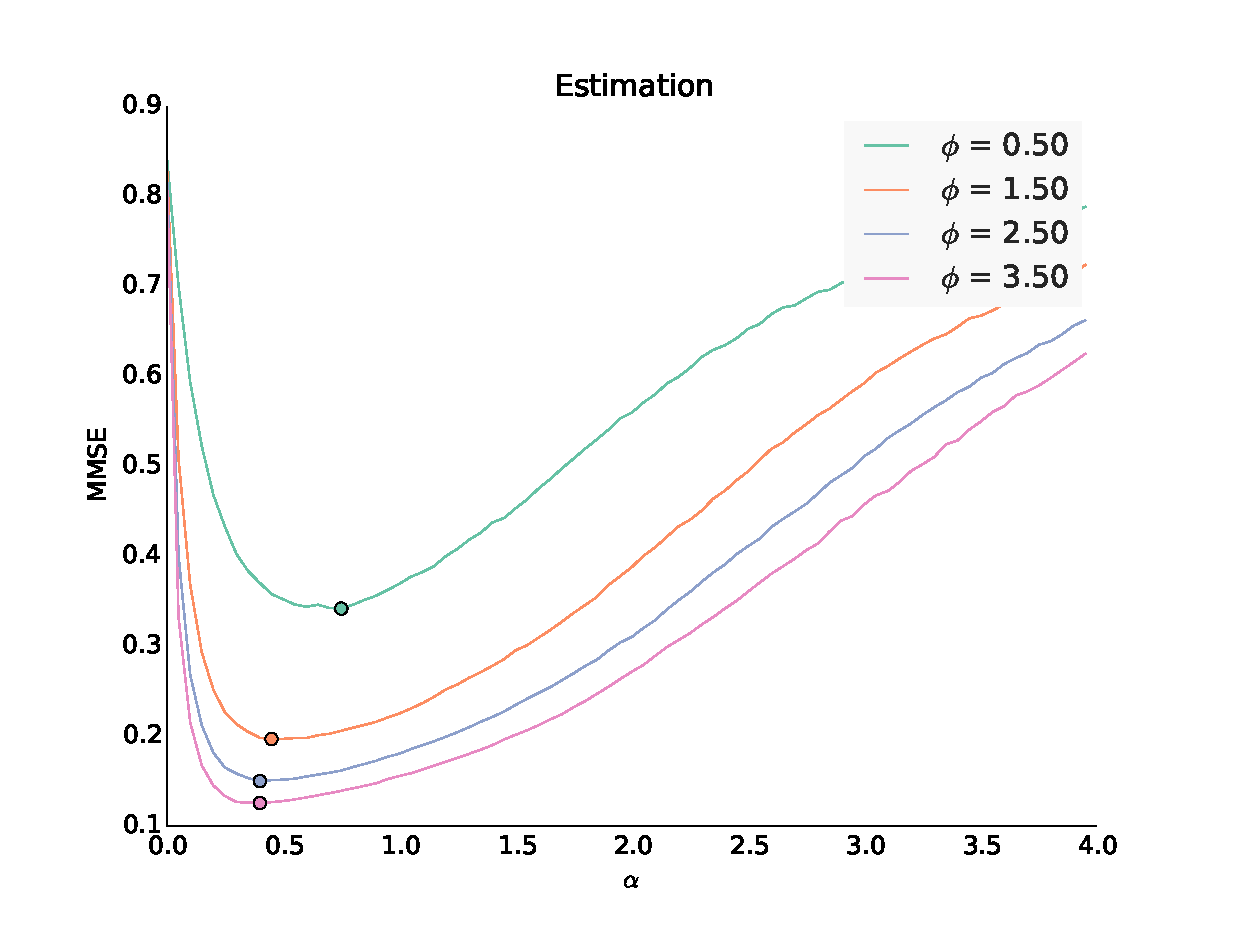
\includegraphics[width=\columnwidth]{figures/figure_5_12_a.eps}
\caption[MSE for the filtering of bistable processes.]{Dependence of the MSE on the tuning width $\alpha$. The width follows the same trend as for the previously considered processes.
The tuning width decreases with increasing firing rates. However, here one can see, that the minimum is less sharp, due to the bistable nature of the process. If a spike allows one
to discern between the two stable states, it already contributes a lot to the estimation of the state $X(t)$.}
\end{figure}

\section{Optimal Codes for Control}

\label{sec:optimal_code_control}

I have extensively argued for the usefulness of accurate estimation of a system's state when interacting with it. Though this is by no mean false, real world
systems are often very high-dimensional, or at least represented in a very high-dimensional code, leading to trade-offs when deciding where to allocate sensory
resources. One simple example is the density of photoreceptors in the retina. If we assume the retina evolved to allow for optimal estimation of the visual scene
facing an animal, we would expect it to cover the entire visual field evenly. That is of course not the case, and there are a number of anomalies in the distribution
of receptive fields which can be attributed to the importance of different visual queues for decision making and risk assessing. A simple example of which is the distribution of photoreceptors in the retina, with the concentration of cones varying up to two orders of magnitude between the periphery and the fovea.\mycite{curcio1987}
\par

What could be the reasons for an optimal code for an estimation problem to be sub-optimal for a control problem? I will present examples that show two possible
reasons for different optimal coding strategies in estimation and control. First, one should note that control problems are often defined over a finite time horizon. One
set of classical experiments involves reaching for a target under time constraints.\mycite{Battaglia2007} If one takes the maximal firing
rate of the neurons ($\phi$) to be constant while varying the width of the tuning functions, this will lead the number of observed spikes to be inversely proportional to
the precision of those spikes, forcing a trade-off between the number of observations and their quality. This trade-off can be tilted to either side in
the case of control depending on the information available at the start of the problem. If one is given complete information on the system state at the initial time $0$,
the encoder needs fewer spikes to reliably estimate the system's state throughout the duration of the control experiment,
and the optimal encoder will be tilted towards a lower number of spikes with higher precision.
Conversely, if at the beginning of the experiment one has very little information about the system's state, the encoder will be
forced towards lower precision spikes with higher frequency.\par

Secondly, one should note that the optimal encoder for estimation does not take into account the differential weighting of different dimensions of the system's state.
When considering a multidimensional estimation problem, the optimal encoder will generally allocate all its resources equally between the dimensions of the system's
state. In the framework presented below one can think of the dimensions as the singular vectors of the tuning matrix $\covar$ and the resources allocated to it as the
singular values. In this sense, I will consider a set of coding strategies defined by matrices $\covar$ of constant determinant.
This constrains the overall firing rate of the
population of neurons to be constant, and one can then consider how the population should best allocate its observations between these dimensions. Clearly, in an
anisotropic control problem, which places a higher importance in controlling one dimension, the optimal encoder for the control problem will be expected to allocate
more resources to that dimension. This is indeed shown to be the case for the Poisson codes considered, as well as for a simple LQG problem with Gaussian observations in 
continuous time when we constrain the noise covariance to have the same structure.\par

\subsection{The Trade-off Between Precision and Frequency of Observations}
\label{sec:information}

In this section I consider populations of neurons with tuning functions as given by \fref{eq:dense_poiss_gauss_tf} having tuning centers $\theta_m$ distributed along a 
one-dimensional line.
In the case of a stimulus modelled by the Ornstein-Uhlenbeck process these will be simply one-dimensional values $\theta_m$ whereas in the case of the stochastic oscillator, I will
consider tuning centres of the form $\theta_m = (\eta_m,0)^\top$, filling only the first dimension of the stimulus space. This means that in the case of the stochastic oscillator, the 
observer does not have direct access to the velocity of the system, only of its position. Note that  in both cases the (dense) population
firing
rate $\hat{\lambda} = \sum_m \lambda_m (x)$ will be given by $\hat{\lambda} = \sqrt{2\pi} \alpha \phi / |\Delta \theta|$, where $\Delta \theta$ is the separation between neighbouring tuning centres $\theta_m$.\par

The OU process controlled by a process $U(t)$ is given by the SDE
\[
dX(t) = (b U(t)-\gamma X(t)) dt + D^{1/2}dW(t),
\]
and the control problem is defined by a cost function
\[
C(X,U) = \int_0^T \left(X(t)^\top Q X(t) + U(t)^\top R U(t)\right)dt.
\]
\Fref{eq:poiss_cost} can then be evaluated by simulating the dynamics of
$\Sigma(t)$. This is exactly the problem solved in \fref{chap:mse} and it has extensively been discussed therein.\footnote{See also \mycitep{Susemihl2013}.}
Following those results one can also approximate the average of the posterior variance by a mean-field formalism which works surprisingly well. The evolution of the 
average posterior variance is given by the average
of \fref{eq:filtering_sde_sigma}, which involves nonlinear averages over the covariances. The mean-field evolution of 
$\boldsymbol{E}\left[\Sigma(t)\middle| \Sigma_0\right]$ is given by
\[
\frac{d\boldsymbol{E}\left[\Sigma(t)\right]}{dt} = A \boldsymbol{E}\left[\Sigma(t)\right] + \boldsymbol{E}\left[\Sigma(t)\right]^\top A^\top + D - \hat{\lambda}  \boldsymbol{E}\left[\Sigma(t)\right]\covar^\dagger  \boldsymbol{E}\left[\Sigma(t)\right] \left(I+\covar^\dagger  \boldsymbol{E}\left[\Sigma(t)\right]\right)^{-1}.
\]
To assess the quality of this approximation I have also computed the averages of $\Sigma(t)$ numerically with a large number of sample paths to compare to the
mean-field approximation. In \mycitep{Susemihl2011a} and \mycitep{Susemihl2013} I had reported a very good agreement in the mean-field and numerically calculated 
values of $ \boldsymbol{E}\left[\Sigma(t)\right]$. $f(\Sigma,t)$ however is an integral over time of this average, so one can expect that the deviation between the mean-field approximation and the 
numerical average will be larger. As can be seen in \fref{fig:comparison_uni}, the mean-field approximation is not as precise as in the case
of the simple average, but the dependence of the average on $\alpha$, however, remains very well explained by the mean-field approach.\par
Alternatively, one can look at a system with more complex dynamics, and I will take as an example the stochastic damped harmonic oscillator given by the system of equations
\begin{equation}
\label{eq:stoch_osc}
\dot{X}(t) = V(t),\quad dV(t)=\left(b U(t)-\gamma V(t)  - \omega^2 X(t) \right)dt + \eta^{1/2} dW(t).
\end{equation}
Furthermore, I assume that
the tuning functions only depend on the position of the oscillator, therefore not giving any information about the velocity. The controller in turn seeks to keep the
oscillator close to the origin while steering only the velocity. This can be achieved by the choice of matrices
\[
A = \left(\begin{array}{cc}0& 1\\ -\omega^2 & -\gamma\end{array}\right), B=  \left(\begin{array}{cc}0& 0\\ 0 & b\end{array}\right), D = \left(\begin{array}{cc}0&0\\ 0&\eta^2\end{array}\right),
\]
\[
R=\left(\begin{array}{cc}0&0\\0&r\end{array}\right), Q = \left(\begin{array}{cc} q& 0\\0& 0\end{array}\right)\textrm{ and } \covar =\left(\begin{array}{cc}\alpha^2&0\\0&0\end{array}\right).
\]\par

In \fref{chap:control} I have argued that a good way to quantify the effect of the encoder on the costs of a control problem is the function $f(\Sigma,t)$ derived there. This quantifies
the effect of the uncertainty resulting from estimating the system's state through that encoder on the control costs.
In \fref{fig:comparison_uni} I have plotted the uncertainty-dependent costs $f$ for LQG control, for the Poisson observed control, as well as the MMSE for the Poisson
filtering problem and for a Kalman-Bucy filter with a same noise covariance equal to the tuning matrix $\covar$. This
illustrates nicely the difference between Kalman filtering and the Gauss-Poisson filtering considered here. The Kalman filter MSE has a simple, monotonically
increasing dependence on the noise
covariance, and one should simply strive to design sensors with the highest possible precision ($\alpha=0$) to minimise the MMSE and control costs. The Poisson case
leads to optimal performance at a non-zero value of $\alpha$. Importantly the optimal values of $\alpha$ for estimation and control differ. Furthermore, in view of
\fref{sec:mutual_info}, I have also
plotted the mutual information between the process $X(t)$ and the observation process $N(t)$, to illustrate that information-based arguments would lead to the same
optimal encoder as MMSE-based arguments.\par

The result that the MMSE-optimal encoder also maximises the mutual information had not been previously reported, and is most likely a consequence of the Gaussian
nature of the distributions considered. It can be shown to hold exactly in the mean-field approximate, as well. The mutual information quantifies the information contained in the observations about the stimulus. The MSE on the other hand
quantifies the second moment of the difference between the estimate and the true value of the stimulus. If all distributions are Gaussian, these two quantities are related
as all the information the observations can contain are condensed into the two first moments of the posterior distribution. This does not need to be the case generally,
but provides an interesting point of entry to further research questions.
\par
\begin{figure}
\includegraphics[width=\columnwidth]{figures/figure_5_13_a.pdf}
\includegraphics[width=\columnwidth]{figures/figure_5_13_b.pdf}
\caption[Trading off precision and frequency in control and estimation problems.]{{The trade-off between the precision and the frequency of spikes is illustrated for the OU process (top) and the stochastic oscillator (bottom). In both figures, the initial condition has a very uncertain estimate of the system's state, biasing the optimal tuning width towards higher values. This forces the encoder to amass the maximum number of observations within the duration of the control experiment. Parameters for figure (a)
were: $T =2,\, \gamma = 1.0,\, \eta = 0.6,\, b = 0.2,\, \phi = 0.1,\, \Delta\theta = 0.05,\, Q = 0.1,\, Q_T = 0.001,\, R = 0.1$.  Parameters for figure (b) were $T=5,\,
\gamma=0.4,\,\omega=0.8,\,\eta = 0.4,\, r=0.4,\, q=0.4,\, Q_T = 0,\, \phi = 0.5,\, \Delta\theta=0.1$.   }}
\label{fig:comparison_uni}
\end{figure}


\subsection{Allocating Observation Resources in Anisotropic Control Problems}
\label{sec:determinant}

A second factor that could lead to different optimal encoders in estimation and control is the structure of the cost function $C$. Specifically, if the cost functions
depends more strongly on a certain coordinate of the system's state, uncertainty in that particular coordinate will have a higher impact on expected future costs than
uncertainty in other coordinates. I will here consider two simple linear control systems observed by a population of neurons restricted to a certain firing rate. This
can be thought of as a metabolic constraint, since the regeneration of membrane potential necessary for action potential generation is one of the most significant
metabolic expenditures for neurons.\mycite{attwell2001energy} This will lead to a trade-off, where an increase in precision in one coordinate will result in a decrease in
precision in the other coordinate.\par

I consider a
population of neurons whose tuning functions cover a two-dimensional space. Taking a two-dimensional isotropic OU system with state $X(t)=(X_{1,t},X_{2,t})^\top$ 
where both dimensions are uncoupled,
one can consider a population with tuning centres $\theta_m = (\eta^m_1,\eta^m_2)^\top$
densely covering the stimulus space. To consider a smoother class of stochastic systems I will also consider a two-dimensional stochastic oscillator with state
$X(t) = (X_1(t),V_1(t),X_2(t),V_2(t))^\top$, where again, both dimensions are uncoupled, and the tuning centres of the form 
$\theta_m = (\eta^m_1, 0, \eta^m_2,0)^\top$, covering densely the position space, but not the velocity space.\par
Since I am interested in the case of limited resources, I will restrict myself to populations with a tuning matrix $\covar$ yielding a constant population firing rate. One
can parametrise these simply as
\[
\covar_{OU}(\zeta) = p^2\left(\begin{array}{cc}\tan(\zeta)&0\\0&\cotan(\zeta)\end{array}\right)
\]
for the OU case and
\[
\covar_{Osc}(\zeta) = p^2\left(\begin{array}{cccc} \tan(\zeta) & 0 &  0\\ 0&0&0&0\\0&0& \cotan(\zeta)&0\\0&0&0&0\end{array}\right)
\]
for the stochastic oscillator, where $\zeta \in (0,\pi/2)$.
This will yield the firing rate $\hat{\lambda} = 2\pi p^2 \phi/(\Delta \theta)^2$, independent of the angle $\zeta$.\par

One can then compare the performance of all observers with the same firing rate in both control and estimation tasks.
As mentioned, I am interested in control problems where the cost functions are anisotropic, that is, one dimension of the system's state vector contributes more
heavily to the cost function. To study this case I will consider cost functions of the type
\[
c(X(t),U(t)) = Q_1 X_1(t)^2+ Q_2 X_2(t)^2 + R_1 U_1(t)^2 +R_2 U_2(t)^2.
\]
This again, can be readily cast into the formalism introduced above, with a suitable choice of matrices $Q$ and $R$ for both the OU process as for the stochastic
oscillator. I will look at the t the case where the first dimension of $X(t)$ contributes more strongly to the state costs (i.e., $Q_1 > Q_2$).

The filtering error can be obtained from the formalism developed in \fref{chap:mse} in the case of Poisson observations and directly from the Kalman-Bucy
equations in the case of Kalman filtering. For LQG control, one can simply solve the control problem for the system mentioned through the Ricatti equation and obtain an
estimate of the uncertainty-related costs (see e.g. \mycitet[p.288]{astrom2006}). The Poisson-coded version of the control problem can be solved using either direct simulation of the
dynamics of $\Sigma(t)$ or by a mean-field approach which has been shown to yield excellent results for the system at hand. These results are summarised in
\fref{fig:comparison_radial}, with similar notation to that in \fref{fig:comparison_uni}. Note the extreme example of the stochastic oscillator, where the optimal encoder
is concentrating all the resources in one dimension, essentially ignoring the second dimension.
\begin{figure}
\includegraphics[width=\columnwidth]{figures/figure_5_14_a.pdf}
\includegraphics[width=\columnwidth]{figures/figure_5_14_b.pdf}
\caption[Differential allocation of observation resources for estimation and control.]{{The differential allocation of resources in control and estimation for the OU process (top) and the stochastic oscillator (bottom). Even though the estimation MMSE leads to a symmetric optimal encoder both in the Poisson and in the Kalman filtering problem, the optimal encoders for the control problem are asymmetric, allocating more resources to the first coordinate of the stimulus.
}}
\label{fig:comparison_radial}
\end{figure}
